
%%%%%%%%%%%%%%%%%%%%%%% file typeinst.tex %%%%%%%%%%%%%%%%%%%%%%%%%
%
% Author: Mauricio Matamoros
% Updated: Oct 31, 2022
% Contact: mauricio@robocupathome.org
%
% This is the LaTeX source for the TDPTemplate using
% the LaTeX document class 'llncs.cls' Springer LNAI format
% used in the RoboCup Symposium submissions.
% http://www.springer.com/computer/lncs?SGWID=0-164-6-793341-0
%
% It may be used as a template for your own TDP - copy it
% to a new file with a new name and use it as the basis
% for your Team Description Paper
%
% NB: the document class 'llncs' has its own and detailed documentation, see
% ftp://ftp.springer.de/data/pubftp/pub/tex/latex/llncs/latex2e/llncsdoc.pdf
%
% Remark: Last page with specs won't be included in Camera ready TDP's.
%
% CHKTEX-FILE 8
% CHKTEX-FILE 13
%
%%%%%%%%%%%%%%%%%%%%%%%%%%%%%%%%%%%%%%%%%%%%%%%%%%%%%%%%%%%%%%%%%%%

\documentclass[runningheads,a4paper]{llncs}

% XeLaTeX support
\usepackage{ifxetex}
\ifxetex%
	\usepackage{fontspec}
	\usepackage{polyglossia}
	\setmainlanguage{english}
\else
	\usepackage[utf8]{inputenc}
	\usepackage[T1]{fontenc}
	\usepackage[english]{babel}
\fi

% Common packages
\usepackage{amsmath}
\usepackage{amssymb}
\setcounter{tocdepth}{3}
\usepackage{url}
\usepackage{float}
\usepackage{titling}
\usepackage{wrapfig}
\usepackage{booktabs}
\usepackage{csquotes}
\usepackage{fancyhdr}
\usepackage{graphicx}
\usepackage{subcaption}
\usepackage{lastpage}
\usepackage[all]{nowidow}
\usepackage[inline]{enumitem}
\usepackage[usenames,dvipsnames]{xcolor}

% Referencing packages
\usepackage{varioref}
\usepackage[hidelinks]{hyperref}
\usepackage[noabbrev,nameinlink]{cleveref}

\usepackage{lipsum}
\newcommand{\mytitle}{Chief Scientist Office 2024 Team Description Paper}
\newcommand{\myauthor}{Takaaki Numai, Airi Yokochi, Joshua Supratman, Tatsuro Sakaguchi, Yushi, Kaida, Gakuto Okamoto}

\newcommand{\robospecs}{%
	\newpage%
	\pagenumbering{gobble}%
	\pagestyle{fancy}%
	\fancyhf{}%
	\lhead{}%
	\chead{\footnotesize\myauthor\ | \footnotesize\mytitle}%
	\rhead{}%
	\rfoot{Robot software and hardware specification sheet}%
}

\newcommand{\BnL}[1][1em]{ \includegraphics[width=#1]{images/bnl.jpg} }







%%%%%%%%%%%%%%%%%%%%%%%%%%%%%%%%%%%%%%%%%%%%%%%%%%%%%%%%%%%%%%%%%%%%%%%%%%%%%%%%%%%%
%
% Title
%
%%%%%%%%%%%%%%%%%%%%%%%%%%%%%%%%%%%%%%%%%%%%%%%%%%%%%%%%%%%%%%%%%%%%%%%%%%%%%%%%%%%%
\title{Chief Scientist Office 2023 Team Description Paper}

\author{Takaaki Numi, \and Airi Yochi, \and Tatsuro Sakachi, \and Yuushi Kaida, \and Gakuto Okanoto, \and Joshua Superman}
\institute{Affiliation name and address, \\
\texttt{http://devoted-web-site.url}}


\begin{document}
\maketitle

%%%%%%%%%%%%%%%%%%%%%%%%%%%%%%%%%%%%%%%%%%%%%%%%%%%%%%%%%%%%%%%%%%%%%%%%%%%%%%%%%%%%
%
% Abstract
%
%%%%%%%%%%%%%%%%%%%%%%%%%%%%%%%%%%%%%%%%%%%%%%%%%%%%%%%%%%%%%%%%%%%%%%%%%%%%%%%%%%%%

\begin{abstract}
	This paper presents SoftBank Corp. Japan team Chief Scientist Office’s new mobile manipulator “SOAR” for RoboCup 2024 @Home Open Platform League.
	Differing from our previous participation with “Cuboid-X,” a robot assembled from commercial products, “SOAR” integrates both custom-developed and commercial components, a significant step toward developing a customizable and affordable robotic platform.
	Our main achievement this year has been the successful integration of various hardware components and software development to tackle RoboCup challenges.

	Our approach includes detailed hardware design and calibration, such as the arm and the sensor-rich head unit.
	The software focuses on developing systems, such as object and speech recognition, tailored to the dynamic environment of RoboCup.

	“SOAR” embodies our vision of a robotic system that combines modularity with cost-effectiveness.
	As we continue to refine SOAR’s capabilities further, we are optimistic about its potential to create an adaptable, cost-effective robotic platform for a variety of applications and fields.

\end{abstract}


%%%%%%%%%%%%%%%%%%%%%%%%%%%%%%%%%%%%%%%%%%%%%%%%%%%%%%%%%%%%%%%%%%%%%%%%%%%%%%%%%%%%

\section{Introduction}
This paper details the RoboCup @Home Open Platform League team Chief Scientist Office from SoftBank Corp. Japan.
This is our second appearance at RoboCup @Home Open Platform League.
Since our last participation in 2022, we have made significant improvements, which include the introduction of our new mobile manipulator “SOAR.”

At SoftBank Corp. Chief Scientist Office, we aim to pioneer a customizable and affordable commercial robot platform akin to the modular ease found in computer assembly or the historical T-Ford model.
Our mission is to democratize robotics, making it accessible and adaptable for research and commercial use.
We believe in a future where integrating robotics into business is as straightforward as selecting components for a custom PC build.
With “SOAR” as a stepping stone, we aim to develop a versatile platform that celebrates modularity in both hardware and software, allowing seamless integration and upgrades through a suite of interchangeable modules.

\subsection{Focus of research}
Our research is motivated by the ambition to develop a customizable and affordable robot platform.
We recognize the constraints of current technologies and are committed to exploring their limits and potential. Key areas of our interest include but are not limited to:
\begin{itemize}
	\item Modularity and Configurability: Investigate how to design a system that allows for easy integration and customization of hardware modules.
	\item Technological Feasibility: Assessing the capabilities of existing technologies to meet our affordability and performance criteria.
	\item Device Integration: Tackling the hardware challenges related to the seamless integration of diverse devices and components
	\item Software Optimization: Addressing the limitation of current software modules, such as MoveIt, by enhancing computation speed and completing critical functions.
\end{itemize}
We believe that these research areas are crucial to bridging the gap between the aspirational and the practical, laying the groundwork for a robot that can adapt to various needs.

\section{Hardware}
“SOAR” is a mobile manipulator comprising of four main components; the mobile base, the manipulator, the torso unit, and the head unit.
The mobile base and the manipulator are commercially available products while the torso and head units are developed in-house and designed by our team.
The hardware is designed with a modular approach so that it not only facilitates customization but also simplifies maintenance and upgrades, allowing for the interchange of components as needed.
Fig. \ref{fig:soar_overview} shows the the image of “SOAR.”

\begin{figure}[tbp]
	\centering
	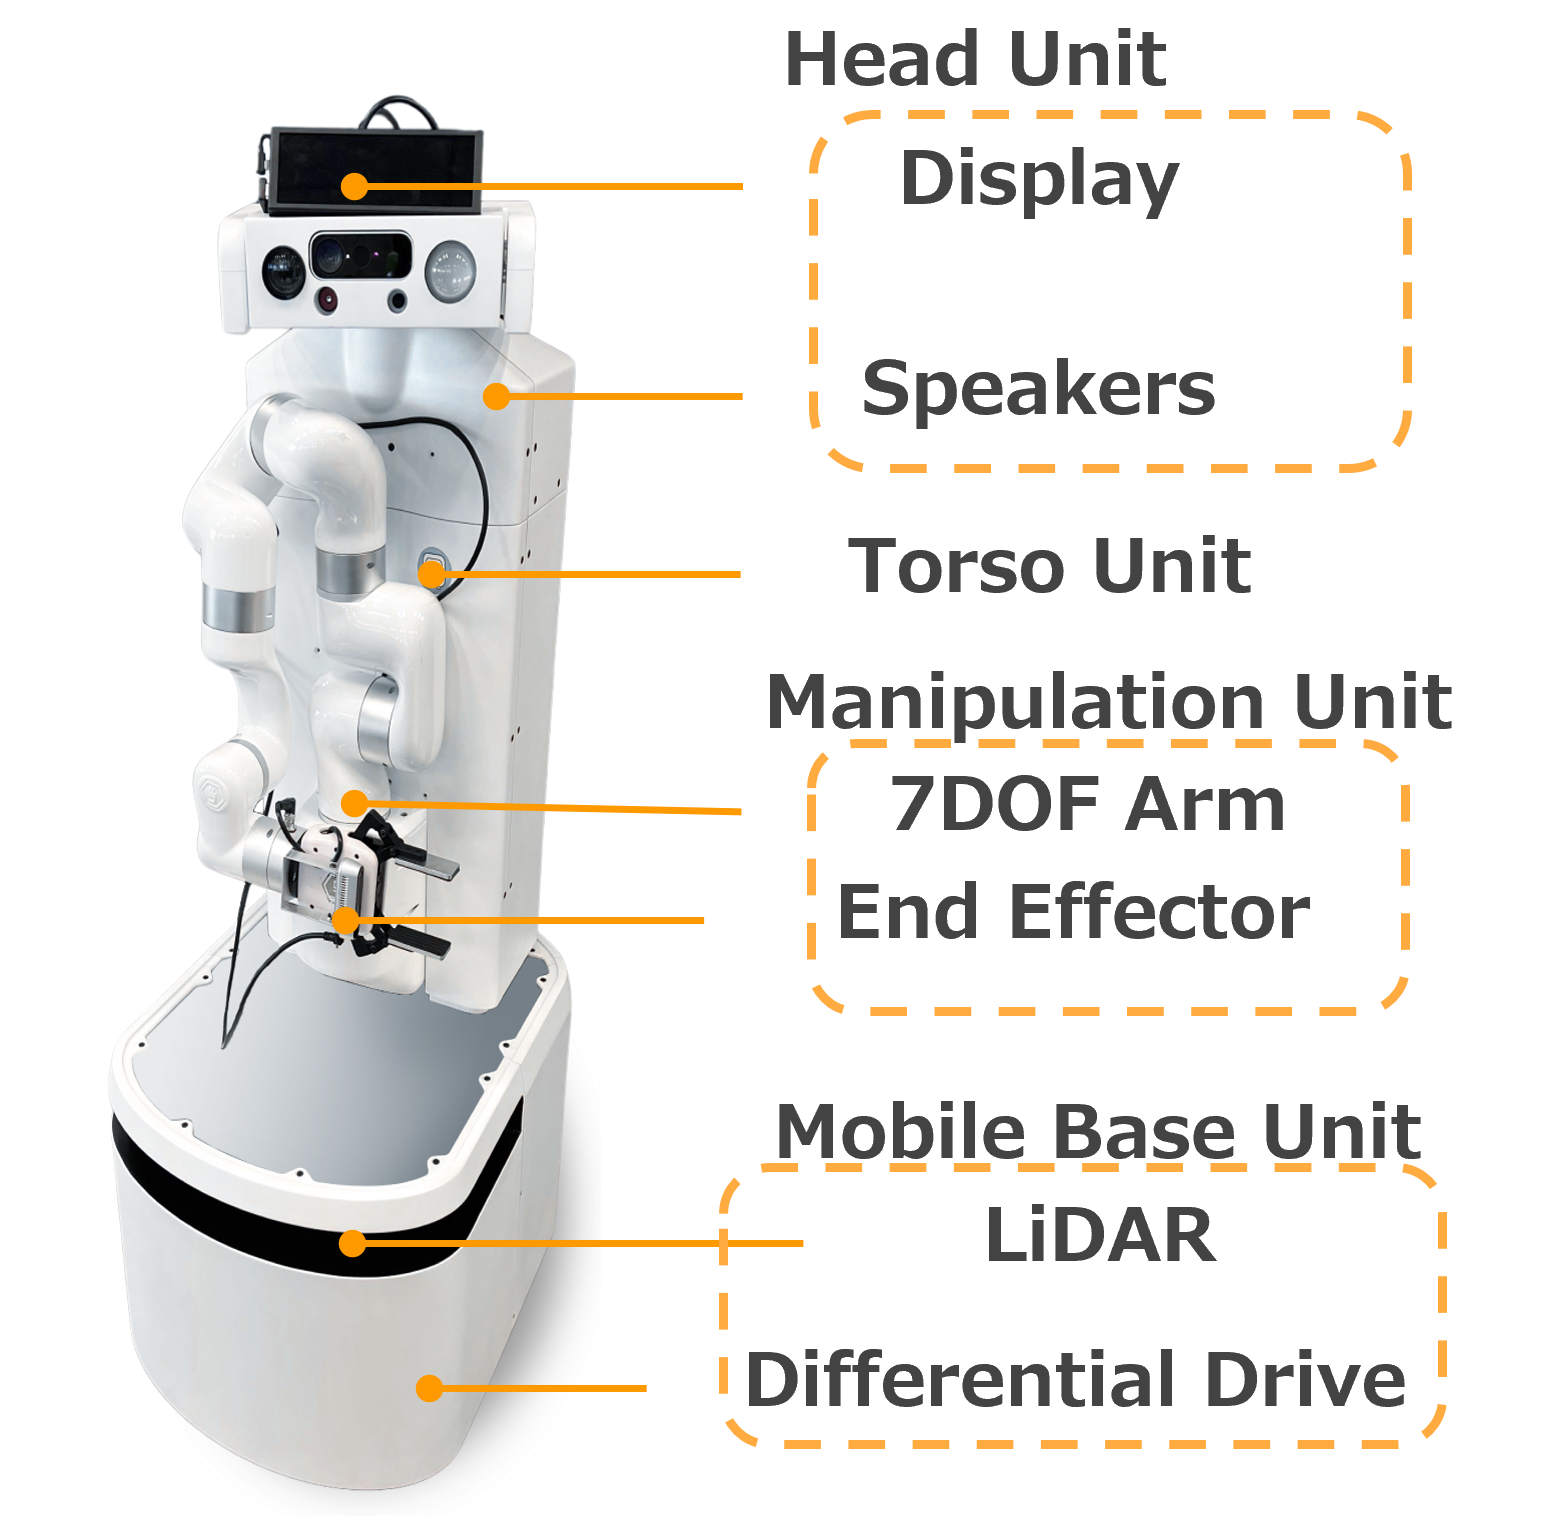
\includegraphics[width=0.5\linewidth]{images/soar_overview.png}
	\caption{Image of SOAR.}
	\label{fig:soar_overview}
\end{figure}

\subsection{Mobile Base}
SOAR’s mobile base is a 2-wheel differential drive mobile base developed by F-Design\footnote{\url{https://f-ds.jp/}}.
It is supplemented with two casters and each driving wheel and caster are equipped with suspensions for smoother movement and stability.
The base has a maximum speed of 3.0 km/h.
We made additional modifications to the unit, equipping it with a LiDAR and an IMU sensor for navigation.
We also integrated a docking charging connector, enabling SOAR to autonomously recharge its batteries once depleted, enhancing its operational autonomy and efficiency.

\subsection{Torso and Manipulator}
SOAR’s arm is composed of two units; the torso and the manipulator.
The manipulator is xArm 7\footnote{\url{https://www.ufactory.cc/xarm-collaborative-robot/}}, a commercially available product developed by uFactory.
It has seven degrees of freedom with a payload of 3.5 kg.
The torso unit, developed by our team, is a linear actuator with one degree of freedom.
The torso unit elevates the manipulator, providing a clearance of 460 mm, which significantly enhances the arm’s reach and versatility.
The end-effector is equipped with a two-finger gripper and a RGB-D hand camera.

\subsection{Head Unit}
The head unit has two main purposes: recognizing and understanding the environment and facilitating social interaction with people.
The head unit is a hub of sensory and interactive technology, equipped with various devices including a RGB-D camera, a zoom camera, a thermal camera, LED lights, a head display, a microphone, and a speaker.
The device placement is shown in Fig. \ref{fig:head}
Additionally, the head has 2 degrees of freedom for pan and tilt movements, enhancing its SOAR’s ability to survey diverse environments and engage in social interaction more effectively.

\begin{figure}[tbp]
	\centering
	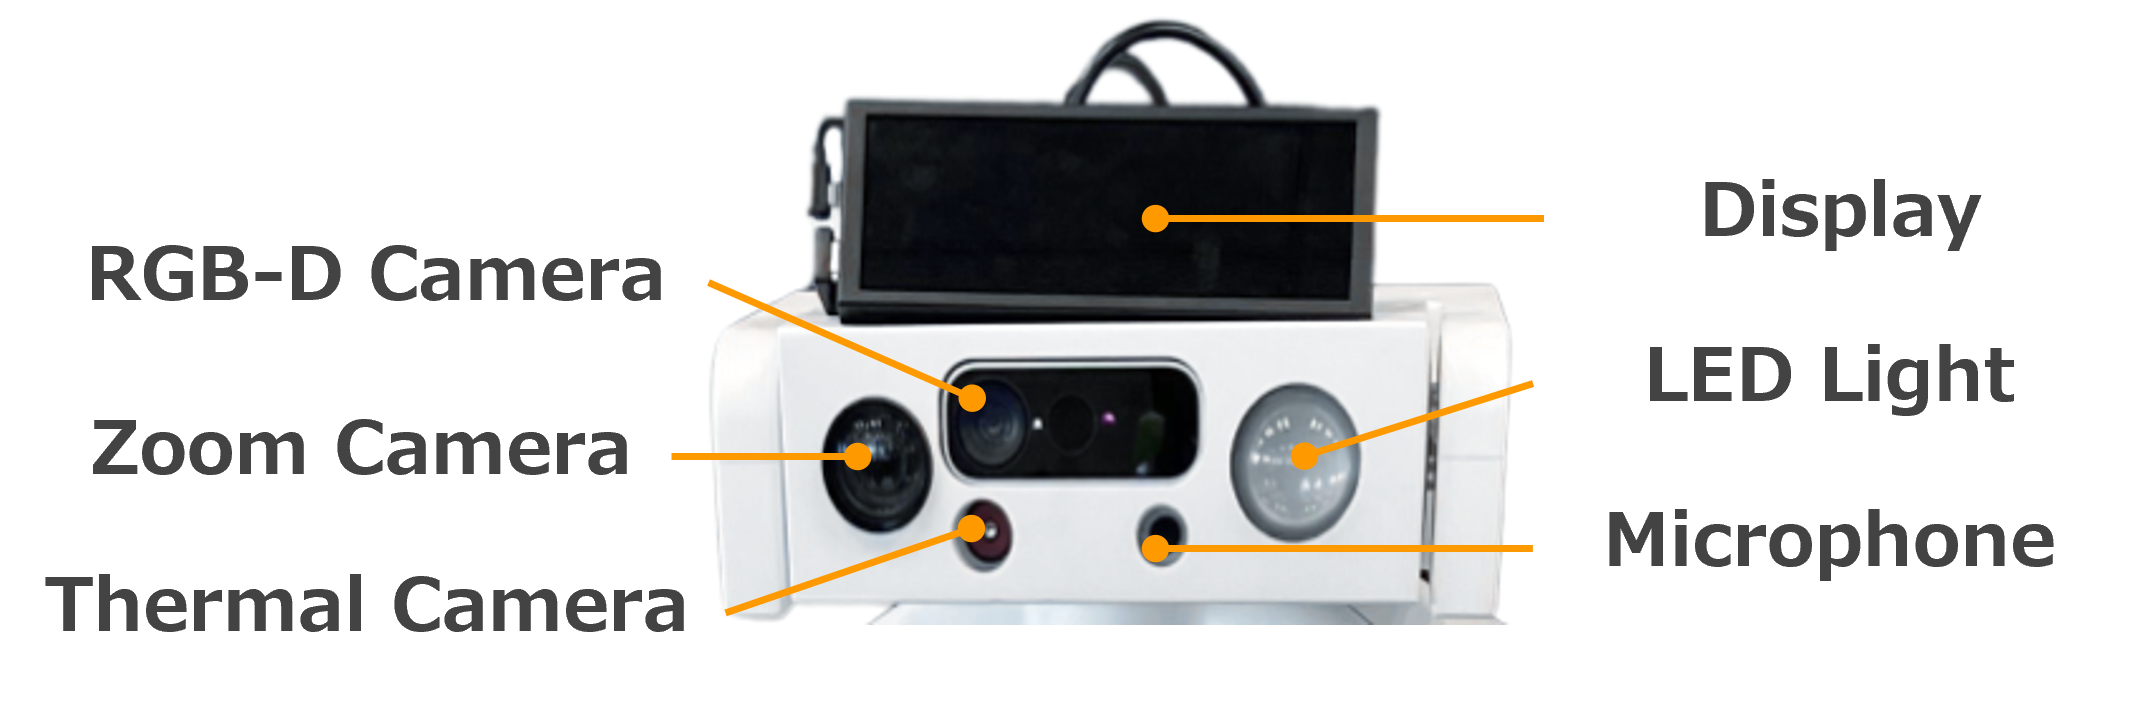
\includegraphics[width=1.0\linewidth]{images/head_unit.png}
	\caption{Device placement on the head unit.}
	\label{fig:head}
\end{figure}

\subsection{Calibration}
SOAR’s design incorporates interchangeable modules like the manipulation unit.
This, however, brings forth unique calibration challenges.
These challenges arise due to alignment issues, accuracy demands, adaptability needs, and the importance of consistent performance across different modules.
Calibration, therefore, becomes essential to ensure that each module functions correctly within the system.

To address this, we employ the \text{robot\_calibration}\cite{ferguson2015robust} ROS package.
This package allows us to fine-tune the arm, aligning the measured joint values with their actual physical counterparts, ensuring accuracy.
While we achieved good calibration results for the manipulator unit, as shown in Fig. \ref{fig:calibration}, the task is more challenging for the head unit and is still undergoing refinement to reach the desired level of accuracy.

\begin{figure}[tbp]
	\centering
	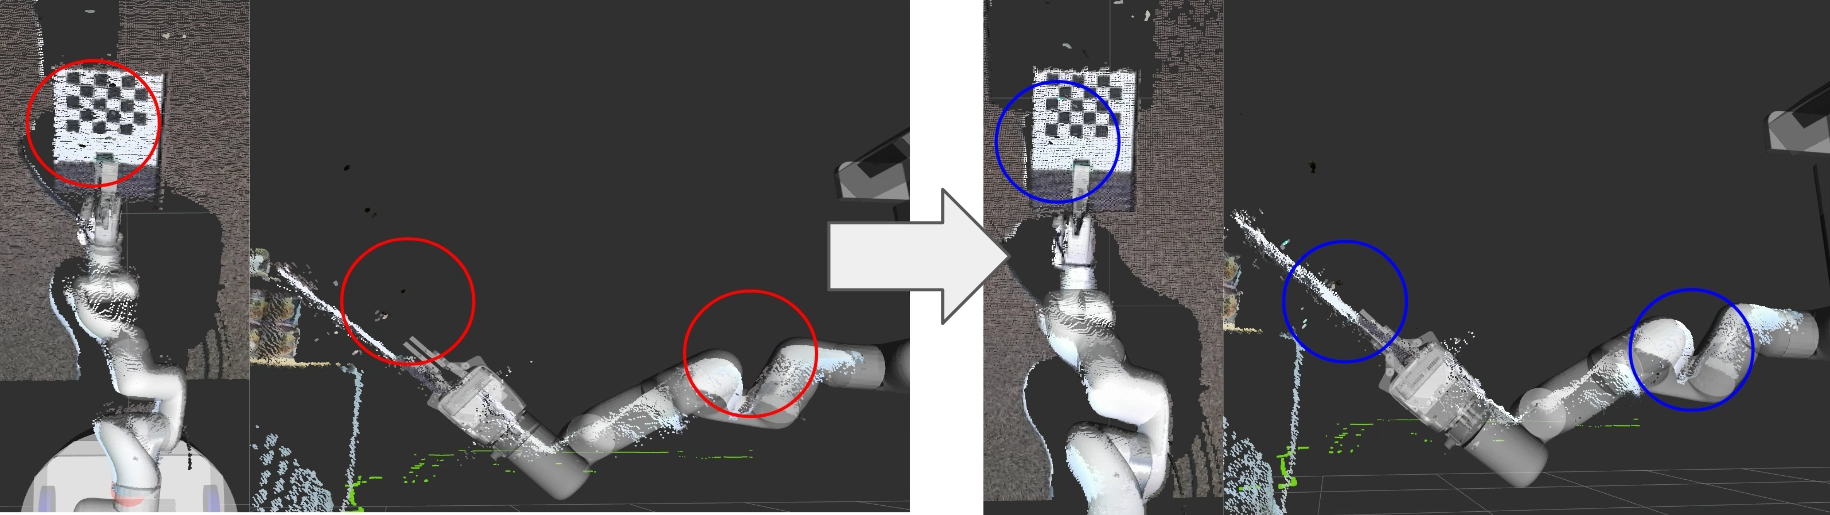
\includegraphics[width=1.0\linewidth]{images/calibration.png}
	\caption{Calibration results. Left show the discrepancies between the measured joint and the actual joint. Right shows the measured
		joint and actual joint after calibration.}
	\label{fig:calibration}
\end{figure}

\section{Software}
The overview of our software system, shown in Fig. \ref{fig:overview} is comprised of three main layers:
\begin{enumerate}
	\item The perception layer, a collection of software modules that take the robot’s sensor data and process them to create a symbolic representation of the environment,
	\item the planning layer, a collection of software modules that take the state of the environment to evaluate and generate a sequence of appropriate robot behaviors, and
	\item the control layer, the collection of software modules that translates the planned behavior and sends appropriate commands to the actuators for the robot to interact with the environment
\end{enumerate}
The primary framework for software module interaction is Robot Operating System (ROS), with each software module representing one or several ROS nodes.

\begin{figure}[tbp]
	\centering
	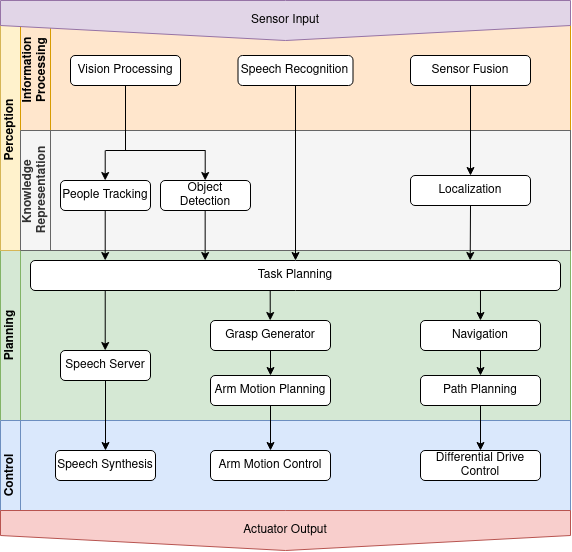
\includegraphics[width=0.7\linewidth]{images/software_overview.png}
	\caption{SOAR software overview.}
	\label{fig:overview}
\end{figure}

\subsection{Object Recognition}
Object detection and 3D localization are handled through the seamless integration of existing technologies.
We employed ultranlytics’s YOLO v8\cite{yolov8_ultralytics} for its object recognition capabilities, producing bounding boxes with labels for each detected object in the robot’s field of view.
To understand the object’s spatial orientation and structure, we used the \text{jsk\_pcl\_ros}\footnote{\url{https://github.com/jsk-ros-pkg/jsk\_recognition}} package for its robust point cloud processing.
We used the EuclideanClustering and the ClusterPointIndices functionalities within this package to segment and cluster point cloud data within the detected bounding boxes from YOLO v8 and generate 3D collision boxes along with its pose.
The pipeline is illustrated in Fig. \ref{fig:object_detection_pipeline}.
\begin{figure}[tbp]
	\centering
	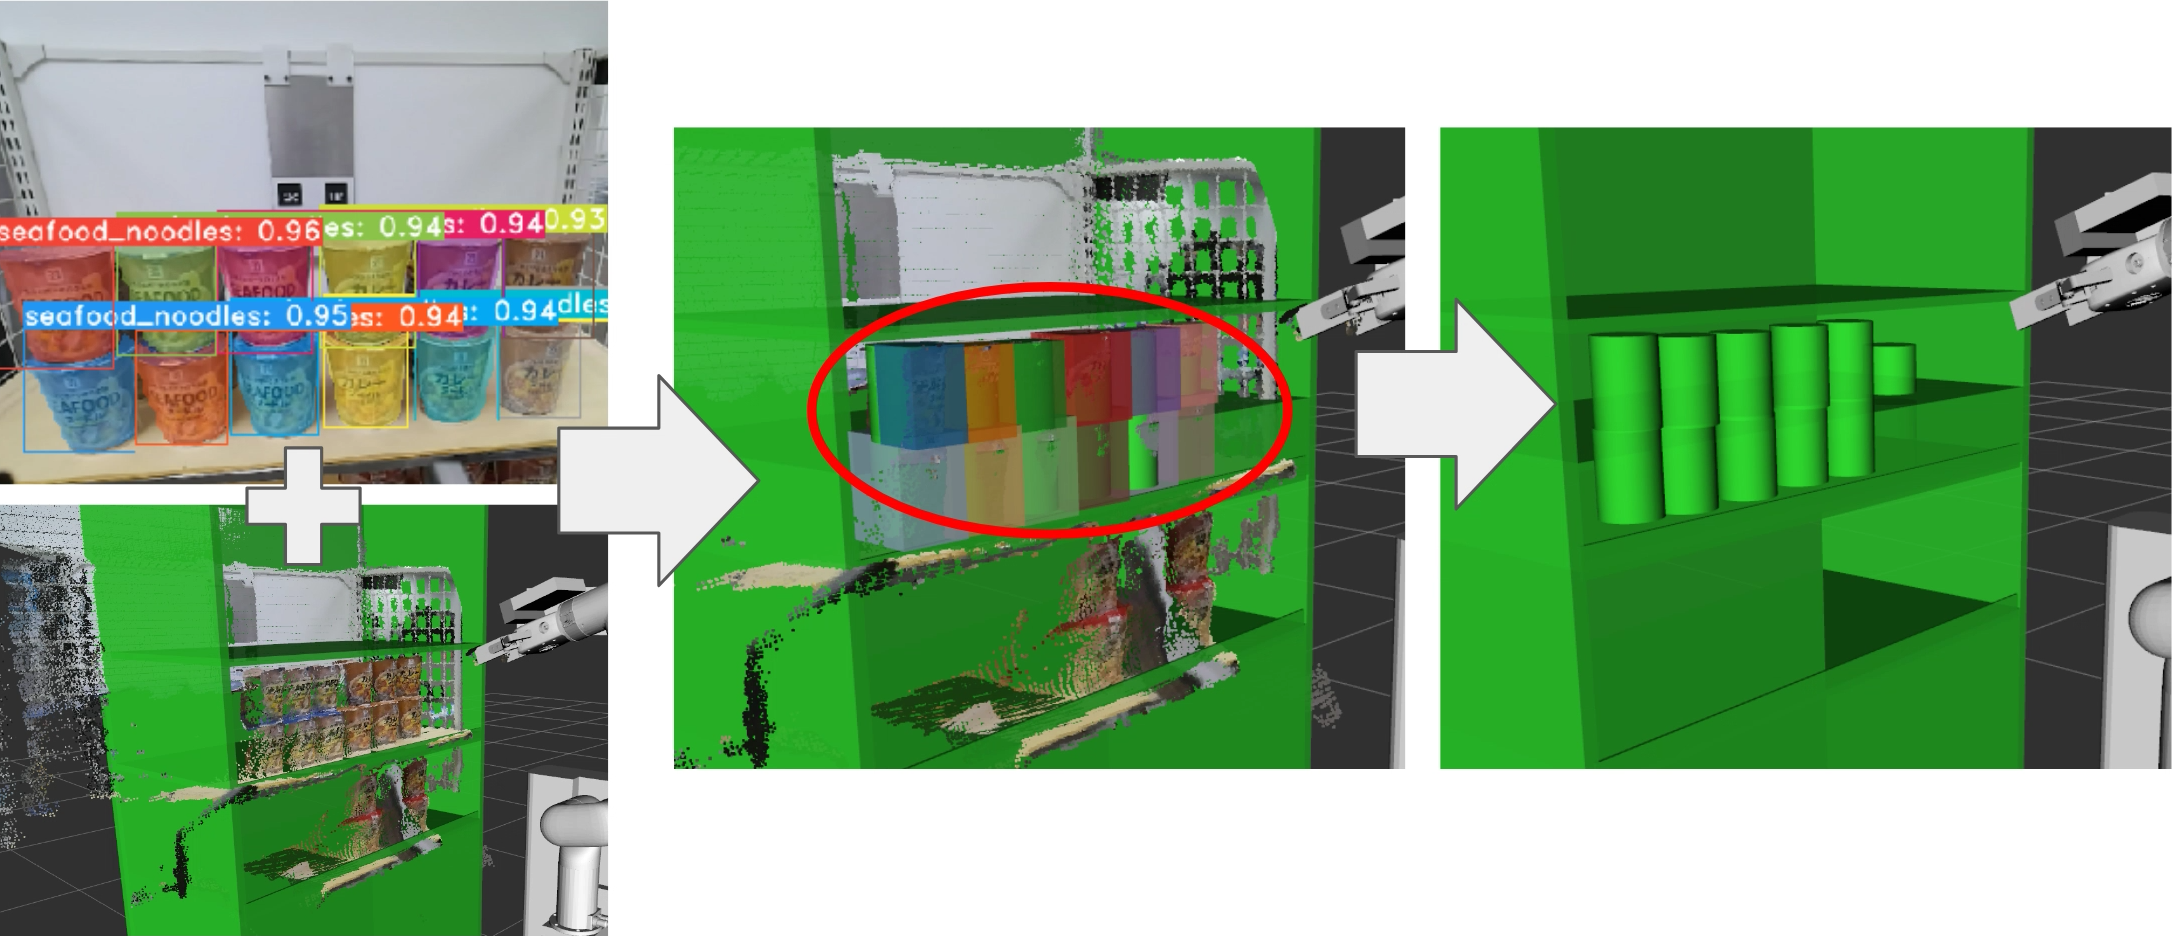
\includegraphics[width=1.0\linewidth]{images/object_detection_pipeline.png}
	\caption{Object detection pipeline.
		YOLO v8's bounding boxes and the point cloud data are given to \text{jsk\_pcl\_ros} package to generate 3D collision boxes which are passed to MoveIt planning scene.}
	\label{fig:object_detection_pipeline}
\end{figure}

\subsection{Creating dataset}
To train YOLO v8 for object recognition in the dynamic nature of RoboCup competitions, where new objects are often introduced on the day of the event, our team has developed a robust method for dataset preparation.
The process involves capturing images of objects from multiple angles and capturing background images on the RoboCup field.
We then crop the object images using a GUI tool and overlay them onto the background images, creating composite images.
We then generate a COCO-style dataset with the composite images.
An example is shown in Fig. \ref{fig:dataset}.
This method significantly simplifies the annotation process, allowing us to create datasets with new objects within a day, thus enabling rapid adaptation and expansion of our object recognition system.

We are continuously working to enhance our model’s capability to recognize challenging objects, such as transparent objects or surfaces with reflective properties like silver.
We are also refining our data collection techniques to consider factors such as varying camera angles and light intensities, which are critical not only for realistic and effective annotation but also for creating 3D simulation models.
These improvements are aimed at increasing the robustness and accuracy of our object recognition system under varied and unpredictable competition conditions.

\begin{figure}[tbp]
	\centering
	\begin{subfigure}[b]{0.8\linewidth}
		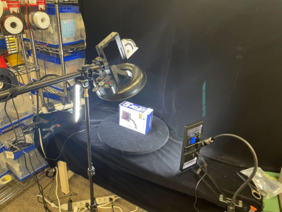
\includegraphics[width=1.0\linewidth]{images/dataset1.png}
		\caption{Use turn-table to capture images of objects from multiple angles and crop the object images using GUI.}
	\end{subfigure}
	\vfill
	\begin{subfigure}[b]{0.8\linewidth}
		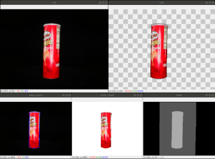
\includegraphics[width=1.0\linewidth]{images/dataset2.png}
		\caption{Generate composite images and used them as dataset for object recognition.}
	\end{subfigure}
	\caption{Dataset creation process.}
	\label{fig:dataset}
\end{figure}

\subsection{Speech Recognition And Interaction}

We use EfficientWord-Net\cite{efficientnet} to detect hotword to initiate the conversion.
Once engaged, we employed Google Dialogflow for conversation, which can interpret spoken phrases and generate relevant responses based on our predefined conversational settings.
For vocal output, we use gTTS\footnote{\url{https://github.com/pndurette/gTTS}} to convert text to speech.

In addition to the current pipeline, we are also exploring the integration of ChatGPT\cite{openai2023gpt4} as a potential replacement for Google Dialogflow to enrich SOAR’s conversational capabilities.
To facilitate this transition, we use Silero VAD\cite{SileroVAD} to segment the voice signals and Whisper\cite{radford2022robust} to convert speech to text.


\section{Contribution}
SoftBank Corp. has continued to sponsor various robotic competitions\footnote{\url{https://wrs.nedo.go.jp/en/sponsor2020/}}\footnote{\url{https://tsukubachallenge.jp/2023/organization/sponsors}} and conferences\footnote{\url{https://ac.rsj-web.org/2023/}}\footnote{\url{https://roscon.ros.org/jp/2023/}} to advocate human-robot interaction research.
Our sister company, SoftBank Robotics Corp. is a long-term global sponsor for RoboCup, which further exemplifies our commitment to advancing robotic technologies and education.
Despite our low direct scientific contribution, SOAR, our current prototype, represents our venture into supporting the research community and industry by offering a platform for research and study.
While it is still in development, SOAR is designed with the future in mind, a testament to our initiative in paving the way for affordable and customizable robots, which we believe will make significant contributions to both academic research and practical applications.

\section{Conclusions and future work}
In this paper, we presented our currently developing robot SOAR which will participate in the RoboCup@Home Open Platform League.
We detailed the hardware specification and introduced several software modules, such as object recognition and speech recognition, which we will continue to refine to tackle the tasks in RoboCup @Home for our future work.
By enhancing SOAR’s capabilities in real-world interaction, we aim to contribute not just a flexible and affordable platform but also a robust platform for research and commercial use.


%%%%%%%%%%%%%%%%%%%%%%%%%%%%%%%%%%%%%%%%%%%%%%%%%%%%%%%%%%%%%%%%%%%%%%%%%%%%%%%%%%%%
%
% Bibliography
%
%%%%%%%%%%%%%%%%%%%%%%%%%%%%%%%%%%%%%%%%%%%%%%%%%%%%%%%%%%%%%%%%%%%%%%%%%%%%%%%%%%%%

\bibliographystyle{unsrt}
\bibliography{bibliography}

\clearpage{}

%%%%%%%%%%%%%%%%%%%%%%%%%%%%%%%%%%%%%%%%%%%%%%%%%%%%%%%%%%%%%%%%%%%%%%%%%%%%%%%%%%%%
%
% Robot Specifications
%
%%%%%%%%%%%%%%%%%%%%%%%%%%%%%%%%%%%%%%%%%%%%%%%%%%%%%%%%%%%%%%%%%%%%%%%%%%%%%%%%%%%%

\robospecs{}
%CHKTEX-FILE 46

\section*{SOAR Hardware Description}%
\label{sec:annex-OPL}
% In this section briefly describe the software and hardware of the robot

\setlength\intextsep{0pt}
\begin{wrapfigure}[10]{r}{0.3\textwidth}
	\centering
	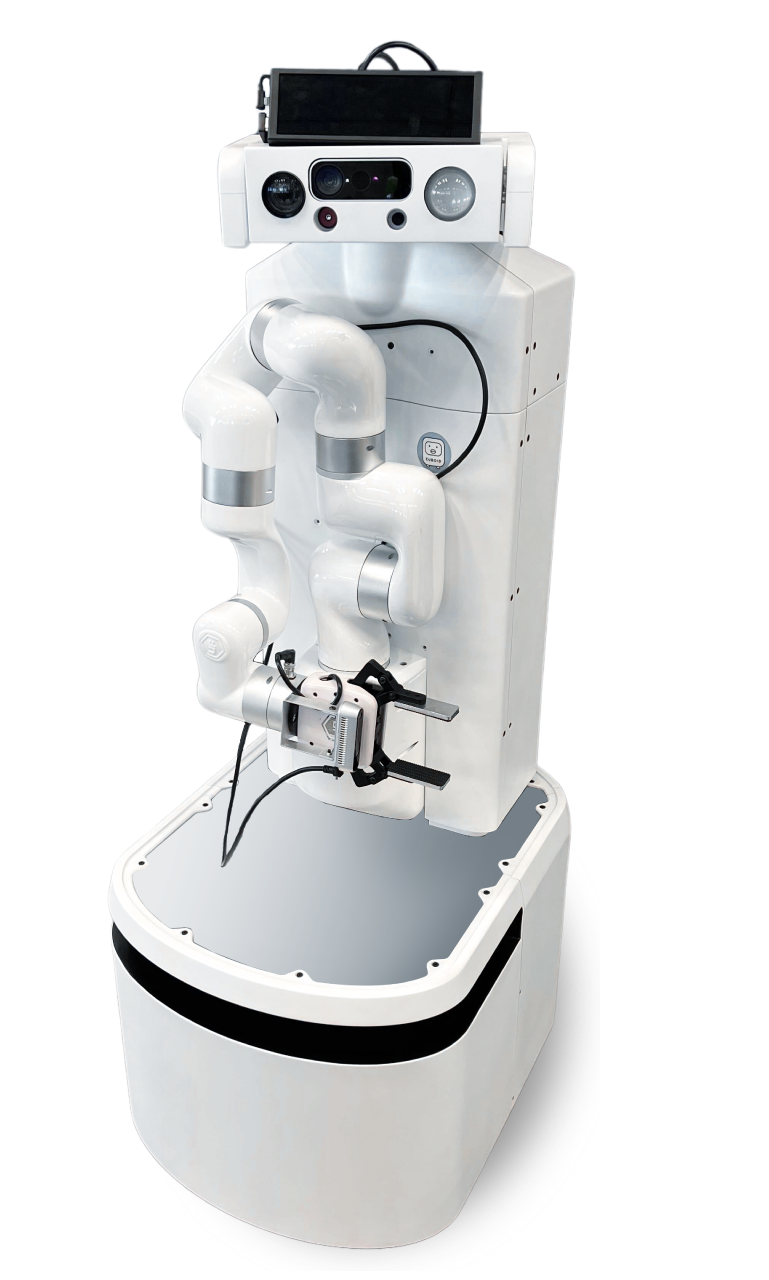
\includegraphics[width=0.4\textwidth]{images/soar.png}
	%\caption{Robot SOAR}%
	\label{fig:soar}
\end{wrapfigure}

Specifications are as follows:

\begin{itemize}
	\item Base: differential drive, 0.83 m/s max speed.
	\item Dimensions: (w) 550 mm (d) 650 mm (h) 1360 mm - 1770 mm
	\item Weight: 92 kg
	\item Arm: 8 DOF (1 DOF torso, 7 DOF manipulator)
	\item Sensors:
	      \begin{itemize}
		      \item Mobile Base:
		            \begin{itemize}
			            \item Hinson LE-50621 LiDAR
			            \item N100 9-axis IMU
		            \end{itemize}
		      \item Head:
		            \begin{itemize}
			            \item Azure Kinect RGB-D camera
			            \item ECM-SP10 microphone
			            \item JM800S-30-360X zoom camera
			            \item Seek Thermal CompactPRO Fast Frame
		            \end{itemize}
		      \item Arm:
		            \begin{itemize}
			            \item Realsense D435 RGB-D camera
		            \end{itemize}
	      \end{itemize}
	\item PC: Intel NUC (NUC11PHKi7C)
	\item Display: THANKO C-79D21B
	\item Speaker: YAMAHA VXS1MLB
\end{itemize}

\section*{SOAR Software Description}
% Please describe in this section the software you are using to control your robot. Consider the following example:

SOAR use the following software components:

\begin{itemize}
	\item Platform: Ubuntu 20.04 ROS Noetic
	\item Navigation: ROS Navigation Stack, EBand local planner
	\item Arm Motion Planner: MoveIt ROS package
	\item Object Recognition:
	      \begin{itemize}
		      \item YOLOv8
		      \item \text{jsk\_pcl\_ros} ROS package
	      \end{itemize}
	\item Behavior Architecture: SMACH ROS package
	\item Hotword: EfficientWord-Net
	\item Speech Recognition: Google Dialogflow
	\item Speech Generation: Google Text-To-Speech
	\item Person Recognition: \text{spencer\_people\_tracking} ROS package
\end{itemize}


\nocite{*}

\end{document}
